\documentclass[a4paper,10pt,titlepage]{article}

\usepackage{geometry}
\usepackage{amsmath}
\usepackage{amssymb}
\usepackage{txfonts}
\usepackage{microtype}
\usepackage{epsfig}
\usepackage{graphicx}
\usepackage{moreverb}
\usepackage{hyperref}
\usepackage{listings}
\usepackage{xcolor}
\usepackage{textcomp}
\definecolor{listinggray}{gray}{0.98}
\definecolor{lbcolor}{rgb}{0.98,0.98,0.98}
\lstset{
	backgroundcolor=\color{lbcolor},
	tabsize=4,
	rulecolor=,
	language=matlab,
    basicstyle=\scriptsize\ttfamily,
    upquote=true,
    aboveskip={1.5\baselineskip},
    columns=fixed,
    showstringspaces=false,
    extendedchars=true,
    breaklines=true,
    prebreak = \raisebox{0ex}[0ex][0ex]{\ensuremath{\hookleftarrow}},
    frame=single,
    showtabs=false,
    showspaces=false,
    showstringspaces=false,
    identifierstyle=\ttfamily,
    keywordstyle=\color[rgb]{0,0,1},
    commentstyle=\color[rgb]{0.133,0.545,0.133},
    stringstyle=\color[rgb]{0.627,0.126,0.941},
}
\usepackage{eso-pic}
\usepackage{ifthen}

\AddToShipoutPictureBG{\ifthenelse{\equal{\value{page}}{0}}{}{
\includegraphics{template_files/backgroundlines}}}

\usepackage{units}
%\usepackage[T1]{fontenc}
%\usepackage[utf8]{inputenc}
\usepackage{physics}

\newcommand{\ee}{\mathrm{e}}
\newcommand{\ii}{\mathrm{i}}
\newcommand{\kB}{k_\mathrm{B}}
\newcommand{\MFT}{\text{MFT}}

\title{H2a: Binary Alloy}
\author{Andr\'eas Sundstr\"om and Linnea Hesslow}
\date{\today}

\begin{document}

\newgeometry{top=2cm,bottom=2cm,left=2cm,right=2cm}

\begin{titlepage}

\setcounter{page}{0}

\begin{center}
{\huge \bf \color{red} NB: The graded, first version of the report must be
                           returned if you hand in a second time! } \\
\vspace{3cm}
\makeatletter
{ \huge \@title } \\
\vspace{1cm}
{ \Large \@author }\\
\vspace{1cm}
{ \Large \@date }\\
\makeatother
\end{center}

\vfill

\begin{flushright}
{\Large
\begin{tabular}{|c|c|c|}
\hline
Task N\textsuperscript{\underline{o}} & Points & Avail.\ points \\ \hline
\hspace{3cm} & \hspace{3cm} & \hspace{3cm} \\ \hline
~ & ~ & ~ \\ \hline
~ & ~ & ~ \\ \hline
~ & ~ & ~ \\ \hline
~ & ~ & ~ \\ \hline
~ & ~ & ~ \\ \hline
~ & ~ & ~ \\ \hline
~ & ~ & ~ \\ \hline
$\sum$ & ~ & ~ \\
\hline
\end{tabular}}
\end{flushright}

\end{titlepage}

\newgeometry{top=2cm,bottom=2cm,left=1.5cm,right=7.4cm}


\section*{Introduction}
Both the mean field theory and the Ising model play an important role in statistical mechanics. We use these two models to study a simple model of a binary alloy of \unit[50]{\%} copper and \unit[50]{\%} zink, commonly known as brass. Some properties of the system can be easily determined in the mean field theory, but a numerical simulation of the Ising model gives more accurate results. Here, we compute various statistical properties and compare the results of the Ising model and the mean field theory.


In both the mean field theory and the Ising model, we model the binary alloy with a static, three-dimensional  bcc lattice  consisting of Cu and Zn atoms. Each atom has eight bonds to each nearest neighbor, with bond energies
\begin{equation}
\begin{aligned}
E_{\rm CuZn} &= \unit[-294]{meV}, \\
E_{\rm CuCu} &= \unit[-436]{meV}, \\
E_{\rm ZnZn} &= \unit[-113]{meV}.
\end{aligned}
\label{eq:energies}
\end{equation}

\section*{Task 1: mean field theory}
In the mean field theory (MFT) model, every individual atom is assumed
to interact only with an average of the whole system, and the system
is also assumed to be in equilibrium. All microscopic
variations are therefore neglected.

In this binary alloy model, we have two sub-lattices (one
Cu~sub-lattice and one Zn~sub-lattice) and we can define an order
parameter
\begin{equation}
P=2\frac{\tilde{N}}{N}-1,
\end{equation}
where $\tilde{N}$ is the number of Cu atoms in the Cu lattice and $N$
is the total number of Cu atoms---equivalently, we could say that $N$
is the number of lattice sites in the Cu~sub-lattice and that
$\tilde{N}/N$ is the fraction of the atoms in the sub-lattice which
are Cu. This order parameter can now be used to define the mean field
theory of this system.

At first, we need a connection between the order parameter, $P$, and the
temperature, $T$. To get to this we note that the equilibrium of the
system is given by minimizing the Helmholz's free energy,
$F_{\MFT}=U_{\MFT}-TS_{\MFT}$, where $U_{\MFT}=E_{\MFT}(P)$ is the
system energy and $S_{\MFT}=\kB\ln\omega_{\MFT}$ is the 
entropy, where $\omega_{\MFT}=\omega_{\MFT}(P)$ is the number of possible
micro-states. In the Cu sub-lattice, there are $\tilde{N}=(1+P)N/2$ Cu
atoms;
% and $N-\tilde{N}=(1-P)N/2$ Zn atoms,
therefore, the number of micro-states in the Cu sub-lattice is
\begin{equation}
\omega_{\MFT}' = {N \choose \tilde{N}} 
= \frac{N!}{\tilde{N}!\,(N-\tilde{N})!}
= \frac{N!}{[(1+P)N/2]!\,[(1-P)N/2]!}
\end{equation}
and the entropy of the Cu sub-lattice is
\begin{equation}
\begin{aligned}
S_{\MFT}'=&\kB \ln(\frac{N!}{[(P+1)N/2]!\,[(P-1)N/2]!})\\
\approx& N\kB\ln(2)
- \kB\frac{N}{2}\Big[(1+P)\ln(1+P) + (1-P)\ln(1-P)\Big],
\end{aligned}
\end{equation}
where Stirling's formula has been used to arrive at the last result.
Now, the Zn sub-lattice is equivalent to the Cu sub-lattice but with
the number Zn atoms and Cu atoms interchanged. The two lattices must
therefore have the same entropies, and the full system entropy is ust
the sum of its parts; hence
\begin{equation}
S_{\MFT}= 2N\kB\ln(2)
- N\kB\Big[(P+1)\ln(1+P) + (1-P)\ln(1-P)\Big].
\end{equation}

Next, we need to find $E(P)$. Using the mean field approximation that
every atom only interacts with the system average, we can derive the
number of the different types of bonds. The number Cu-Cu bonds,
$N^{(\MFT)}_{\rm CuCu}$, are given by the number of Cu atoms in the Cu
sub-lattice, $\tilde{N}$, times the number of bonds each atom has,
$8$, times the probability that another Cu atoms is located in the Zn
sub-lattice\footnotemark{}, $(N-\tilde{N})/N=(1-P)/2$. This 
gives
\footnotetext{This is because bonds can only be made between atoms in
  different sub-lattices.} 
\begin{equation}
N^{(\MFT)}_{\rm CuCu}=8\frac{(1+P)N}{2}\,\frac{1-P}{2}
=2N(1-P^2).
\end{equation}
For the Zn-Zn bonds the number has to be the same, since the Zn and Cu
atoms are interchangeable:
\begin{equation}
N^{(\MFT)}_{\rm ZnZn}=N^{(\MFT)}_{\rm CuCu}=2N(1-P^2).
\end{equation}
Then we know that the total number of bonds in this system has to be
$8N$, and therefore the remaining $8N-N_{\rm ZnZn}-N_{\rm CuCu}$ bonds
has to be inter-species bonds:
\begin{equation}
N^{(\MFT)}_{\rm CuZn}=4N(1+P^2). \label{eq:N_AB}
\end{equation}
The energy of the system is now given by
\begin{equation}
E_{\MFT} = E_{\rm CuZn}N^{(\MFT)}_{\rm CuZn}
+ E_{\rm ZnZn}N^{(\MFT)}_{\rm ZnZn}
+ E_{\rm CuCu}N^{(\MFT)}_{\rm CuCu}, \label{eq:energy}
\end{equation}
which can be simplified to
\begin{equation}\label{eq:E_MFT}
E_{\MFT}(P) = (E_0 - 2P^2\Delta{E})N
\end{equation}
where
\begin{equation}
\begin{aligned}
&E_0=2(E_{\rm CuCu}+E_{\rm ZnZn}+2E_{\rm CuZn}) = \unit[-2.274]{eV},\\
&\Delta{E}=(E_{\rm CuCu}+E_{\rm ZnZn}-2E_{\rm CuZn}) = \unit[39]{meV},
\end{aligned}
\end{equation}
and where
the bond energies are given in equation~\eqref{eq:energies}. We can now find the equilibrium $P=P_{\rm eq}$
by minimizing the free energy
\begin{equation}\label{eq:free-energy}
\begin{aligned}
F_{\MFT}(P,T)=&NE_0 - 2NP^2\Delta{E}\\
&-2N\kB T\ln(2)
+ N\kB T\Big[(P+1)\ln(1+P) + (1-P)\ln(1-P)\Big]\\
=& NE_0 - N\Delta{E}
\qty(2P^2+2\bar{T}\ln(2)
- % Linnea added this factor! 
 \bar{T}\Big[(P+1)\ln(1+P) + (1-P)\ln(1-P)\Big]),
\end{aligned}
\end{equation}
where $\bar{T}=\kB T/\Delta{E}$.

\subsubsection*{The critical temperature}
The critical temperature can be found by differentiating~\eqref{eq:free-energy} with respect to $P$:
\begin{equation}
\begin{aligned}
0 &= \frac{\partial F_{\MFT}(P,T)}{\partial P} \\&=  -4 PN + N \bar T \left[\ln(1+P) + \frac{1+P}{1+P}- \ln(1-P) - \frac{1-P}{1-P}\right] .
\end{aligned}\label{eq:dFdP}
\end{equation}
Equation~\eqref{eq:dFdP} is always fulfilled for $P = 0$, which means that the free energy has a local extremum point at $P = 0 \, \forall \bar T$.  
By expanding~\eqref{eq:dFdP} at small $P$, we find 
\begin{equation}
0 = -4 P + 2 \bar T_{\rm crit} P \rightarrow \bar T_{\rm crit} = 2. \label{eq:Tcrit}
\end{equation}
This means that $\bar T_{\rm crit} = 2$ is the only extremum point at small $P$. We note that
\begin{equation}
\begin{aligned}
 \frac{\partial^2 F_{\MFT}(P,T)}{\partial P^2}\big|_{P=0} 
 %& =  -4 N + N \bar T \left(\frac{1}{1+P} + \frac{1}{1-P} \right) \\
&= 
2N (\bar T-2)  \Rightarrow \begin{cases}
P = 0  \textrm{ minimum if } \bar T > 2 \\
P = 0  \textrm{ maximum if } \bar T < 2. \end{cases}  
\end{aligned}\label{eq:d2FdP2}
\end{equation}
Consequently, there is a phase transition $\bar T = \bar T_{\rm crit} = 2$: the equilibrium order parameter $P \neq 0$ for $\bar T < 2$, whereas $P = 0$ for $\bar T > 2$.

\subsubsection*{Numerical calculations}
To actually minimize \eqref{eq:free-energy} with respect to $P$ for a
given $T$, we need to employ numerical methods. We implemented this in
\textsc{Matlab} and used the \texttt{fminbnd} function to find the
minimum in the range $P\in[0,1]$. This would then give us $P$ as a
function of temperature, $P(T)$. With that, we can the easily
numerically calculated the system energy $U(T)=E(P(T))$ and heat
capacity 
\begin{equation}\label{eq:C_MFT}
C(T)=\pdv{U}{T}=\pdv{E}{P}\pdv{P}{T}.
\end{equation}



\subsubsection*{Results and discussion}
\begin{figure}[!ht]
\begin{center}
  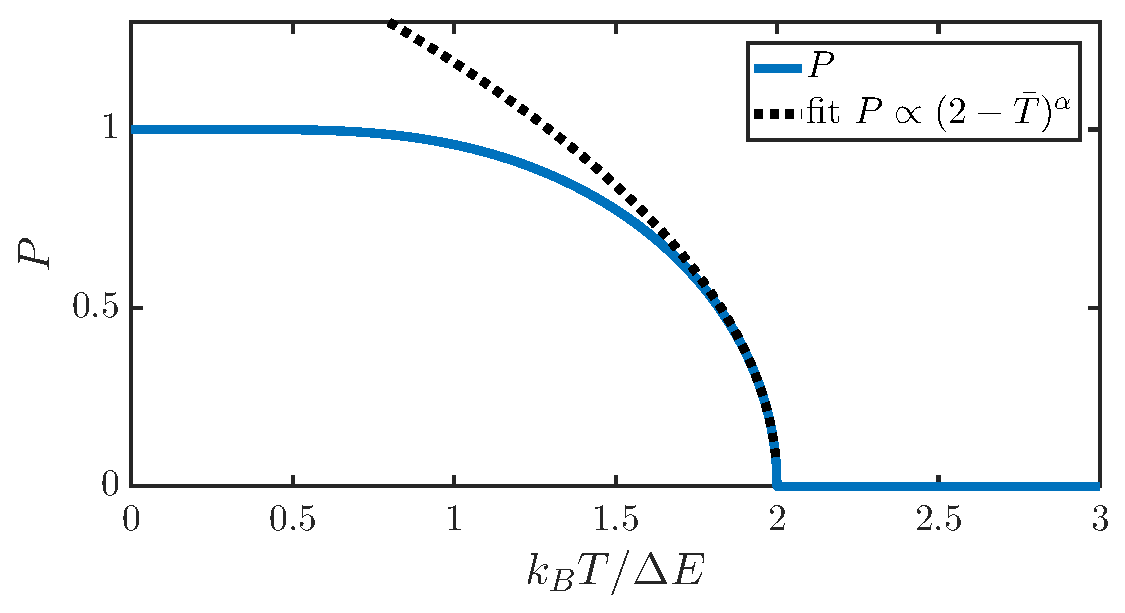
\includegraphics[width=0.7\textwidth]{../figures/P_MFT} 
  \caption{The mean field theory value of the order parameter, $P$, as
  a function of temperature, $\bar{T}=\kB T/\Delta{E}$. There is a
  clear critical temperature, $\bar{T}_{\rm crit}=2$
  ($T_{\rm crit}=\unit[441]{K}$), above which $P$ becomes constantly
  zero. Close below the critical temperature, there is a power law for
  $P(\bar{T})\propto(\bar{T}_{\rm crit}-\bar{T})^{\alpha}$, with
  $\alpha=0.494$; this is shown as the black dotted line. }
  \label{fig:T1:P}
\end{center}
\end{figure}

From the numerical minimization of $F_{\MFT}(P,T)$, we obtained $P(T)$
as shown in figure~\ref{fig:T1:P}. There, we clearly see that there is
a critical temperature at $\bar{T}_{\rm crit}=2$, which is consistent with the prediction~\eqref{eq:Tcrit}. Numerically,
\begin{equation}
T_{\rm crit}=\frac{2\Delta{E}}{\kB}
=\unit[441]{K}=\unit[168]{^{\circ}C}.
\end{equation}
Above this temperature the mean field theory predicts that
$P(T>T_{\rm crit})=0$ is constant, which corresponds to a maximally
disordered system. Below the critical temperature $P$ quickly rises to
$P(0)=1$, which is a maximally ordered system. Note, however, that the
sign of $P$ could just as well be flipped since the system is
symmetric under the transformation $P\to-P$ (just switch label on
which sub-lattice is which). There is a symmetry break at $T=T_{\rm
  crit}$, below which the system will spontaneously order itself into
an asymmetric state: $P<0$ or $P>0$.

We can also find an approximating power law near the critical
temperature:
\begin{equation}\label{eq:alpha}
\hat{P}(T)\propto (\bar{T}_{\rm crit}-\bar{T})^{\beta}=(2-\bar{T})^{\beta},
\end{equation}
with a so called \emph{critical exponent}, $\beta$. We used a log-log
fit to find $\beta=0.494$, and the corresponding power relation is
shown as the dotted black line in figure~\ref{fig:T1:P}. 


\begin{figure}[!ht]
\begin{center}
  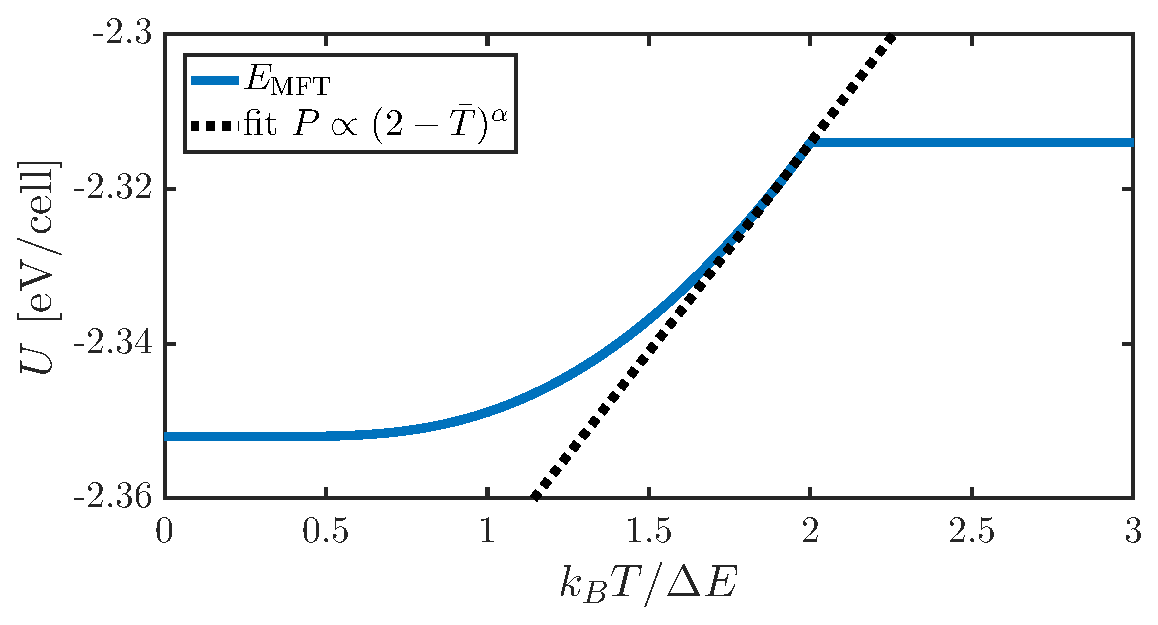
\includegraphics[width=0.7\textwidth]{../figures/E_MFT} 
  \caption{The mean field theory energy per unit cell,
    $u_{\MFT}=U_{\MFT}/N$, as a function of temperature,
    $\bar{T}=\kB T$. The energy rises from
    $u(\bar{T}=0)=E_0-2\Delta{E}=\unit[-2.352]{eV}$ to
    $u(\bar{T}=0)=E_0=\unit[-2.314]{eV}$ per unit cell. }
  \label{fig:T1:E}
\end{center}
\end{figure}

With $P(T)$ found, we can easily use \eqref{eq:E_MFT} to find
$U_{\MFT}(T)=E_{\MFT}(P(T))$, which is plotted in
figure~\ref{fig:T1:E}. There, we see that the energy rises with
temperature, until we reach $\bar{T}=\bar{T}_{\rm crit}=2$ where,
since $P$ becomes constant $P=0$, $U_{\MFT}(T>T_{\rm crit})=N
E_0=-N\times\unit[2.31]{eV}$ becomes constant. We also see that using
the corresponding power law (black dotted line) in $E(\hat{P})$ also
agrees quite well. 

\begin{figure}[!ht]
\begin{center}
  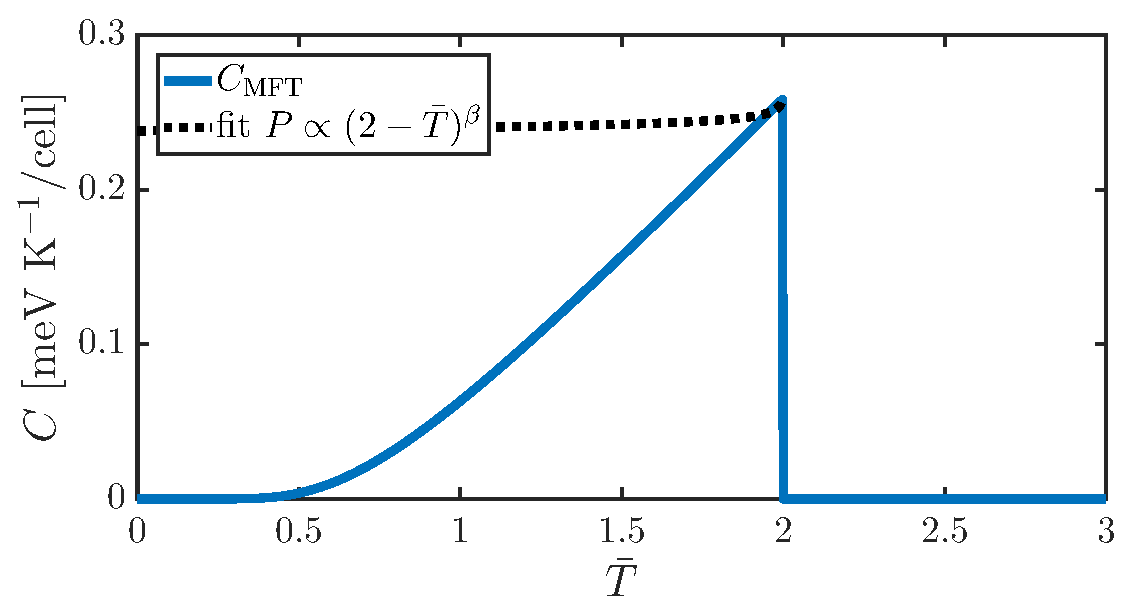
\includegraphics[width=0.7\textwidth]{../figures/C_MFT} 
  \caption{The mean field theory heat capacity, $C_{\MFT}$, as
    function of temperature, $\bar{T}=\kB T/\Delta{E}$. The heat
    capacity rises until $\bar{T}=\bar{T}_{\rm crit}$ to a maximum
    value of about $C_{\MFT}^{(\max)}=\unit[0.26]{meV/K}$ per unit
    cell, above which $C_{\MFT}$ immediately drops to $0$.}
  \label{fig:T1:C}
\end{center}
\end{figure}

Lastly, we can calculate the MFT heat capacity of the system by
numerically differentiate $U$ from before, the result of which is
shown in figure~\ref{fig:T1:C}. Here, we see an almost linear rise in
heat capacity as $T$ approaches $T_{\rm crit}$. Then, above the
critical temperature, the mean field theory heat capacity drops to
$C_{\MFT}(T>T_{\rm crit})=0$. This is clearly not physical since that
would mean that there is no cost in energy to change the temperature
of the system above the critical temperature.

There is also a critical exponent for the heat capacity,
$\hat{C}\propto(\bar{T}_{\rm crit}-\bar{T})^{-\alpha}$. Using
\eqref{eq:C_MFT}, we can easily show that
\begin{equation}
\hat{C}\propto(\bar{T}_{\rm crit}-\bar{T})^{2\beta-1},
\end{equation}
which corresponds to $\alpha=1-2\beta=0.012$. This power law is also
plotted in figure~\ref{fig:T1:C}, but the agreement is much worse than
in the previous two cases.

%The first critical exponent we found, $\beta$, is very close to
%$1/2$ and it is likely that the obtained value deviates from $1/2$
%due to numerical errors. If $\beta=1/2$ exactly, then that would
%correspond to $\alpha=0$, but that is not really what we see in
%figure~\ref{fig:T1:C}.

%By now it is clear that the mean field theory model does not provide a
%very good representation of the physical system and better methods are
%required, such as the numerical simulation in the next task.


%%%%%%%%%%%%%%%%%%%%%%%%%%%%%%%%%%%%%%%%%%%%%%%%%%%%%%%
\section*{Task 2: Ising model}
We use the Metropolis algorithm to estimate statistical properties of the system, which has a size of $10 \times 10 \times 10$ unit cells and periodic boundary conditions. In each simulation step, we swap two randomly selected atoms in the lattice, and determine the energy change $\Delta E$. If 
\begin{equation}
\Delta E \leq 0,
\end{equation}
or if 
\begin{equation}
\exp[-\Delta E/(k_{\rm B} T)] > \xi,
\end{equation}
where $\xi$ is a random number between $0$ and $1$, the change is accepted; otherwise the lattice remains in the previous state for another step. In this way, the Metropolis algorithm allows us to sample the state space according to a probability $p \propto \exp[- E/(k_{\rm B} T)]$, and thus favor the most probable configurations. 

\subsubsection*{Equilibration}
To equilibrate the system, we started with an ordered system and performed $N_{\rm eq, long} = 10^6$ Monte Carlo steps to equilibrate the system at $T = \unit[-200]{^\circ C}$. At higher temperatures, we started with the final lattice state of the previous temperature run, and therefore the number of equilibration steps was reduced to $N_{\rm eq, short} = 5 \cdot 10^5$. For all temperatures, we used $10^7$ Monte Carlo steps in the production run. 

Figure~\ref{fig:T2:equil} shows the equilibration of the energy at three different temperatures: significantly below, close to and significantly above the critical temperature $T \approx \unit[430]{^\circ C}$. 
We note that the energy per unit cell is in the range 
\begin{equation}
E_0 - 2 \Delta E \approx \unit[-2.35 ]{eV}\leq E\leq  E_0  \approx \unit[-2.27]{eV},
\label{eq:E-range}
\end{equation}
which is consistent with the mean field theory prediction~\eqref{eq:E_MFT}; and the energy is equal to or lower than the completely random system where $E = E_0$. 

\begin{figure}[!ht]
\begin{center}
  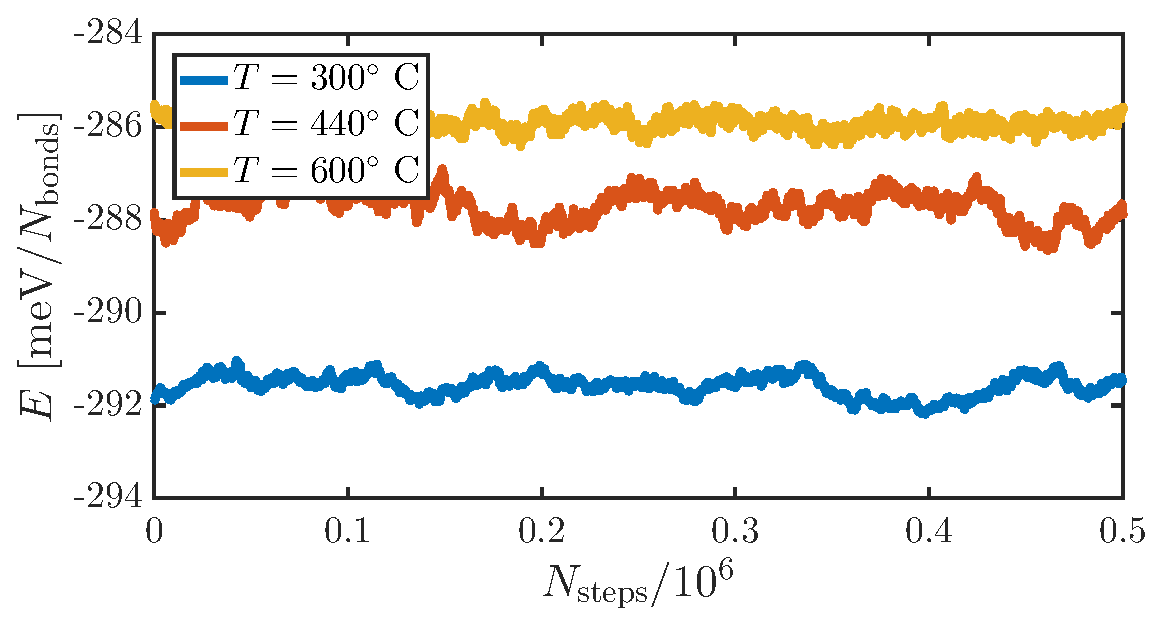
\includegraphics[width=0.7\textwidth]{../figures/equilibration} 
  \caption{The energy per unit cell in the system during the equilibration process.}
  \label{fig:T2:equil}
\end{center}
\end{figure}

\subsubsection*{Statistical properties}
Figure~\ref{fig:U} shows the equilibrium energy per unit cell as a function of temperature, and compared to the mean field theory. We also show the error bars of two standard deviations using the statistical inefficiency  as calculated from the correlation function in section~\ref{sec:ns}. 


\begin{figure}[!ht]
\begin{center}
  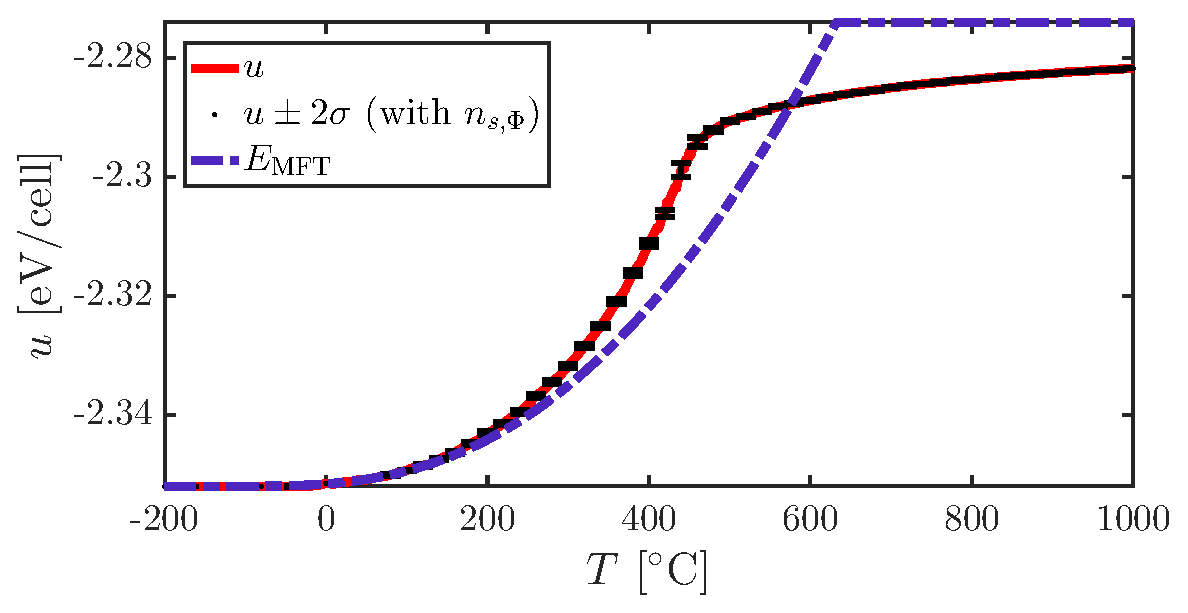
\includegraphics[width=0.7\textwidth]{../figures/U} 
  \caption{The average energy of the system normalized to the number of cells, as a function of temperature. Solid red: simulation, black: error bars at selected temperatures, dash-dotted blue: mean field theory prediction.}
  \label{fig:U}
\end{center}
\end{figure}

The metropolis simulation differs significantly from the mean free theory prediction: the critical temperature is significantly lower in the simulation, and the mean energy continues to increase with temperature beyond the transition. 
In mean field theory, the energy per unit  in the range $u \in [E_0 - 2 \Delta E,  E_0]$ (see equation~\eqref{eq:E-range}. This is fulfilled also in the Monte Carlo simulation, which means that it did not develop clusters of Cu and Zn atoms, in which case the energy per bond would approach the average of the Cu-Cu and Zn-Zn bond energies. In contrast, the simulation does not reach the limit of $u = E_0$ even significantly above $T_{\rm crit}$. 

%In the high temperature limit of an infinite system, the theoretical maximum energy is $ 8 E_{\rm max} \approx \unit[-2.276]{eV}$ (defined in equation~\eqref{eq:Emax}). With a limited system size with 10 cells in each direction, we estimate that the maximum energy should be approximately 
%\begin{equation}
%8 (0.9\cdot E_{\rm max} + 0.1 E_{\rm CuZn}) \approx \unit[2.284]{eV}
%\end{equation}
%Here we obtain $E \approx \unit[-2.287]{eV}$ at $\unit[600]{^\circ C}$, which is slightly below this limit. 

The heat capacity can be determined either by 
\begin{equation}
C = \frac{\partial u}{\partial T},
\label{eq:C1}
\end{equation}
or as the variance in the energy:
\begin{equation}
C = \frac{1}{k_{\rm B} T^2}\left(\langle E^2 \rangle  - \langle E \rangle^2 \right)
\label{eq:C2}.
\end{equation}
Since the latter method does not depend on the derivatives, it gives less noisy data. This is can be seen from figure~\ref{fig:C} by comparing the gray and the black lines. Again, we note that the mean field theory gives a higher critical temperature than the simulation. Moreover, the heat capacity remains non-zero above the critical temperature. Thus, the Ising model does not share  the unphysical artifact of the mean field theory (where there is no cost in energy to change the temperature of the system above the critical temperature). This is because the energy $u < E_0$ even at high temperatures in the simulation. 

\begin{figure}[!ht]
\begin{center}
  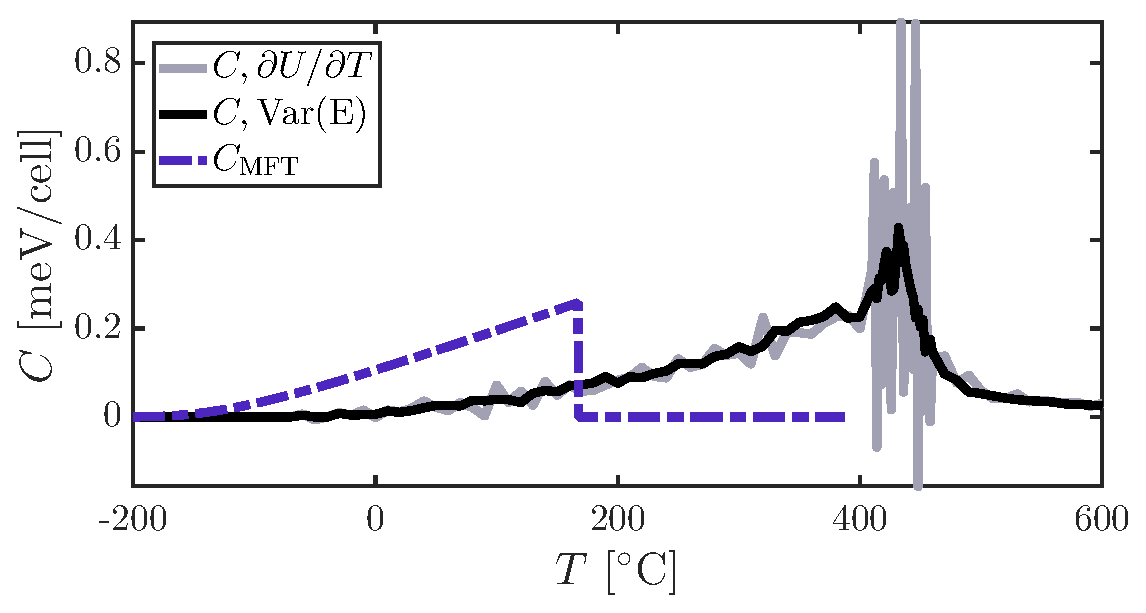
\includegraphics[width=0.7\textwidth]{../figures/C} 
  \caption{The specific heat of the system normalized to the number of cells, as a function of temperature. Solid gray: simulation using the derivative of $U$ directly, black: simulation using the variance of $E$, dash-dotted blue: mean field theory prediction.}
  \label{fig:C}
\end{center}
\end{figure}

\begin{figure}[!ht]
\begin{center}
  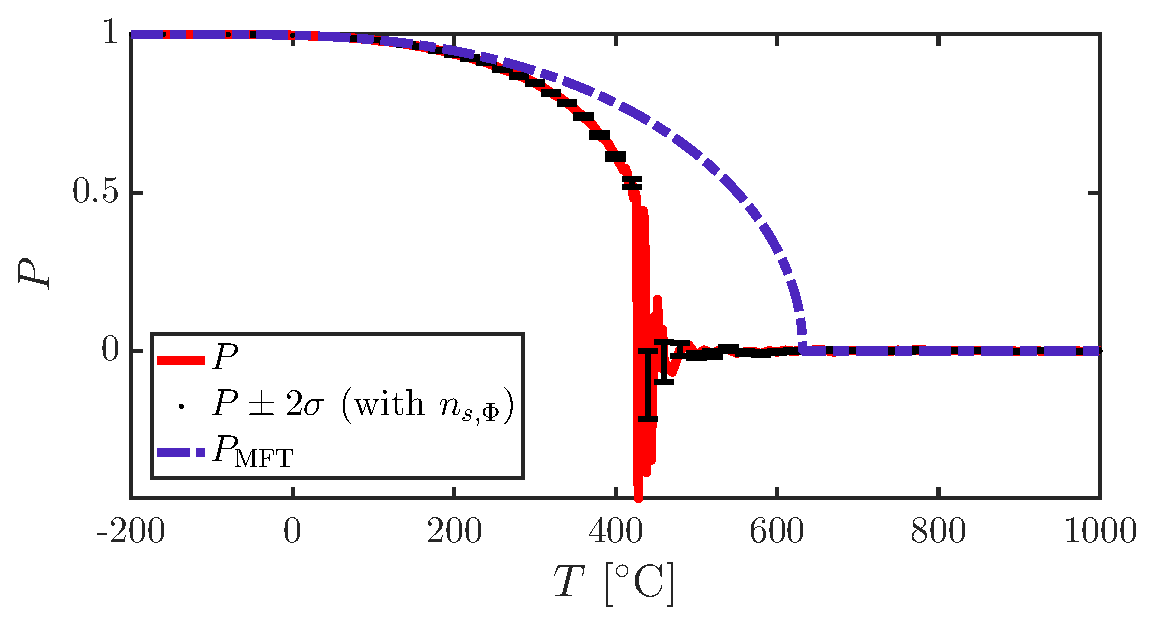
\includegraphics[width=0.7\textwidth]{../figures/P} 
  \caption{The order parameter $P$ as a function of temperature. Solid red: simulation, black: error bars at selected temperatures, dash-dotted blue: mean field theory prediction.}
  \label{fig:P}
\end{center}
\end{figure}

The order parameter $P$ is shown in figure~\ref{fig:P}. Close to the phase transition, the data has high uncertainty, which is also reflected in the large error bars. Note that $P <0$ at some temperatures above the critical temperature -- the system oscillates between a majority of the Cu atoms in the Cu sub-lattice, and a majority in the Zn sub-lattice.  

Finally, the short range order parameter $r$ is determined by the number of nearest-neighbor Cu-Zn bonds as follows
\begin{equation}
r = \frac{1}{4 N}(N_{\rm CuZn}-4N) \rightarrow \begin{cases}
1, \quad& {\rm perfect \, order} \\
0, \quad&  {\rm no \, order, \, homogeneous \, system}\\
-1, \quad& {\rm fully \, separated \, system}
\end{cases}
\end{equation}
In the mean field theory, 
\begin{equation}
r^{\rm MFT} = \frac{1}{4 N}[4N(1+P^2)-4N] = P^2
\end{equation}
by equation~\eqref{eq:N_AB}. Therefore, figure~\ref{fig:r} shows not only the simulation and the MFT prediction, but also the curve $P^2$. Until the transition, $r \approx P^2$ is a good estimation, but at higher temperatures $r$ remains non-zero despite $P \approx 0$. This is a sign that there are still more Cu-Zn bonds than the completely random system. This is also consistent with the energy in figure~\ref{fig:U}, since 
\begin{align}
U &= E_{\rm CuZn}N_{\rm CuZn}
+ \tfrac{1}{2}(8N - N_{\rm CuZn}) ( E_{\rm ZnZn} + E_{\rm CuCu})
%\\&=
% E_{\rm CuZn}4N(r+1)
%+  \tfrac{1}{2}[8N - 4N(r+1) ] ( E_{\rm ZnZn} + E_{\rm CuCu})
\\ &=
 E_{\rm CuZn}4N(r+1)
+ 2N [1 - r] ( E_{\rm ZnZn} + E_{\rm CuCu})  
\\ &=
N E_0   - 2N r \Delta E .
\end{align}
Accordingly, $r = 0$ corresponds to the low temperature limit $u = E_0 -2\Delta E$; the average energy then approaches $u \rightarrow E_0$ at high temperatures (c.f. equation~\eqref{eq:E-range}).   

\begin{figure}[!ht]
\begin{center}
  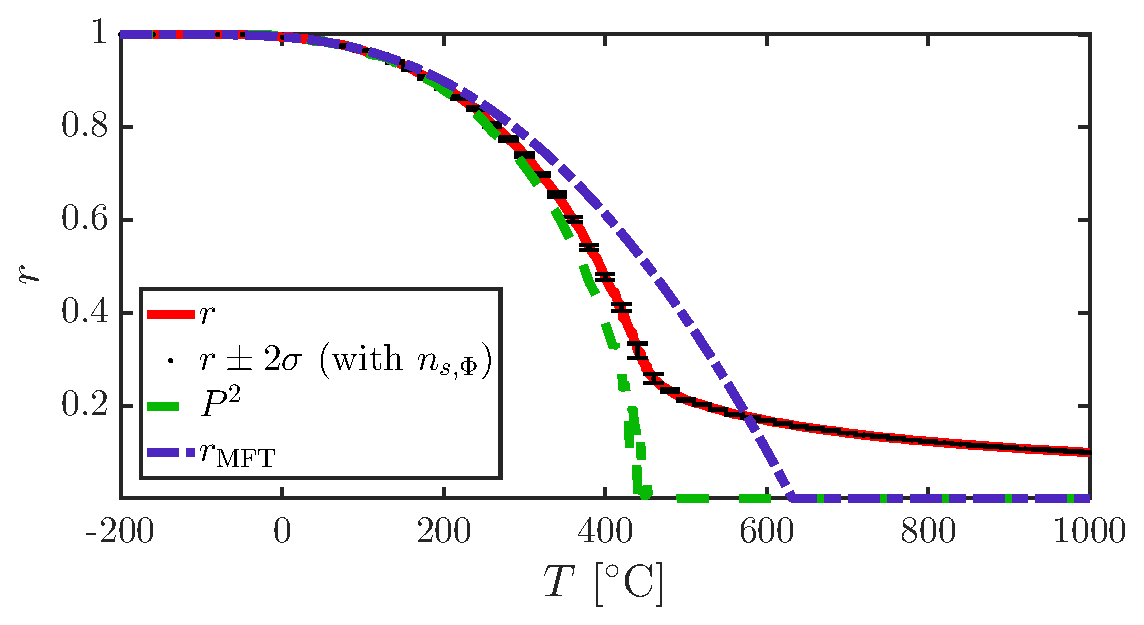
\includegraphics[width=0.7\textwidth]{../figures/r} 
  \caption{The short range order parameter as a function of temperature. Solid red: simulation, black: error bars at selected temperatures, dashed green: estimate $r \approx P^2$, dash-dotted blue: mean field theory prediction. }
  \label{fig:r}
\end{center}
\end{figure}

Finally a note on the critical exponents. Similarly to the MFT analysis, we performed a power law fit of 
the near-critical behavior of $P$ and $C$, resulting in 
\begin{equation}
\beta \approx 0.1, \quad \alpha \approx -0.2.
\end{equation}
Although these values are highly uncertain, we note that the MFT prediction $\alpha_{\rm MFT} = 1-2\beta_{\rm MFT} $ does not generalize to the Ising model simulation. 

\subsubsection*{Statistical inefficiency}
\label{sec:ns}
As described in the Lecture notes, the statistical inefficiency can be used to obtain error estimates of correlated data. 

Suppose we want to measure a quantity $I$, as an average of $N\gg1$ measurements: 
\begin{equation}
I = \langle f \rangle \equiv \frac{1}{N}\sum_{i = 1}^N f_i.
\end{equation}

The variance is then given by 
\begin{equation}
{\rm Var}[I] = \frac{n_s}{N}{\rm Var}[f], \quad {\rm Var}[f] = \langle f^2 \rangle - \langle f \rangle^2,
\end{equation}
where $n_s$ is the statistical inefficiency. 
The statistical inefficiency can be determined either from the decay of the correlation function, 
\begin{equation}
\Phi_{k = n_s} = e^{-2} \approx 0.1, \quad \frac{\langle f_i f_{i+k}\rangle - \langle f \rangle^2}{\langle f^2\rangle - \langle f \rangle^2},
\label{eq:ns_Phi}
\end{equation}
or from block averaging
\begin{equation}
n_s = \lim_{B \rightarrow \infty} \frac{B {\rm Var}[F]}{{\rm Var}[f]}\,, \quad F_j = \frac{1}{B}\sum_{i = 1}^B f_{i + (j-1)B}\,, \quad j \in [1, N_{\rm blocks} ].
\label{eq:ns_block}
\end{equation}

The two methods in equations~\eqref{eq:ns_Phi} and~\eqref{eq:ns_block} should give similar estimates of $n_s$, which they do in the simulations here. The obtained statistical inefficiency is shown in figures~\ref{fig:ns_phi} and~\ref{fig:ns_block}   at three different temperatures, calculated with the correlation function and block average respectively. 

In the case of block average, we used a moving average of 100 points, as the data become noisy when the block size become comparable to the total number of steps. Alternatively, we could have made more blocks of the largest sizes by also using shifted blocks of data, but the results obtained here were considered accurate enough. 

\begin{figure}[!ht]
\begin{center}
  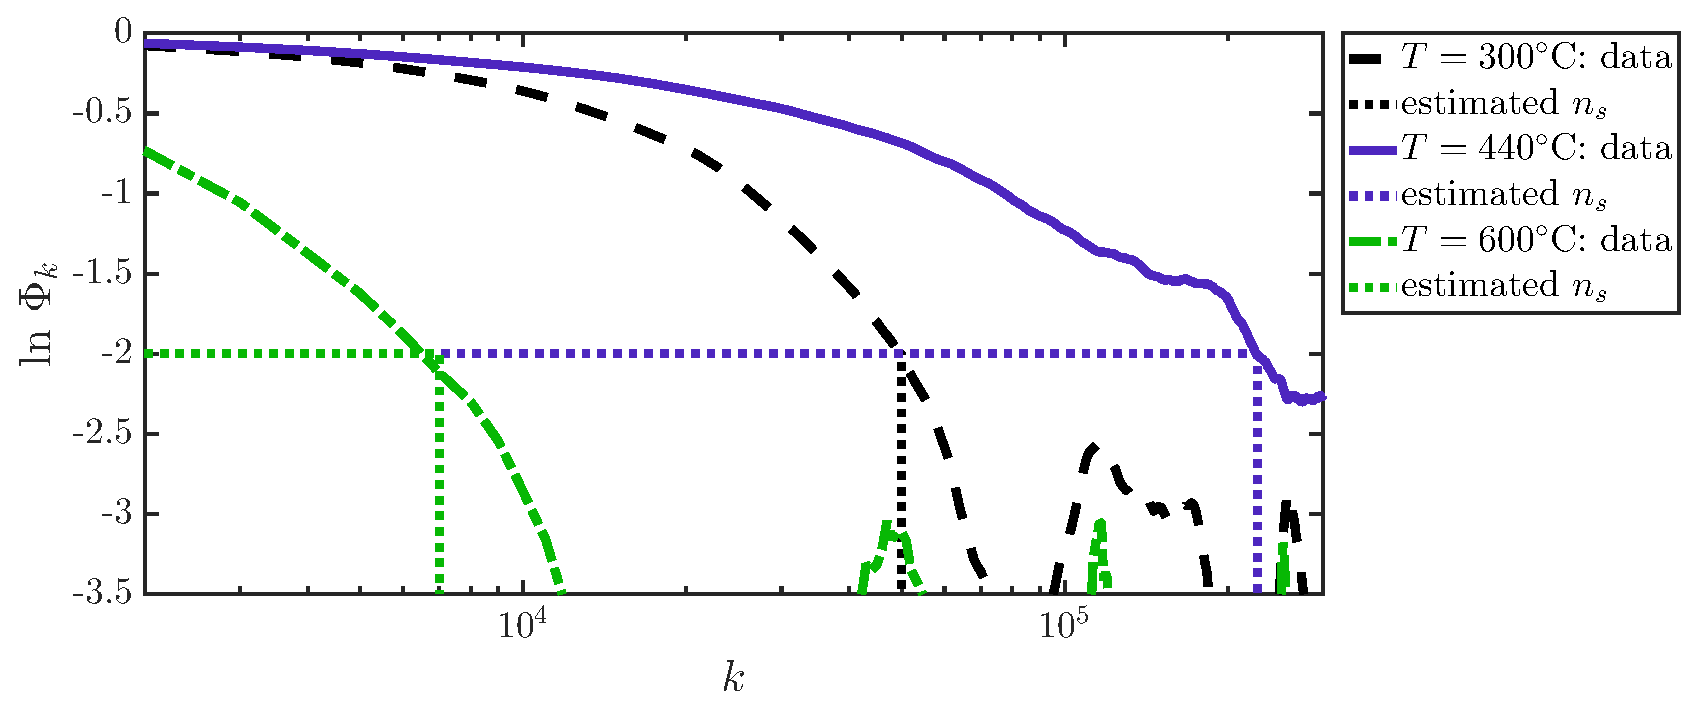
\includegraphics[width=\textwidth]{../figures/stat_inefficiency_Phi} 
  \caption{The logarirhm of the correlation function $\Phi_k(k)$ for three different temperatures. Dotted lines mark the estimated value of $n_s = k (\ln \Phi_k = -2)$.}
  \label{fig:ns_phi}
\end{center}
\end{figure}

\begin{figure}[!ht]
\begin{center}
  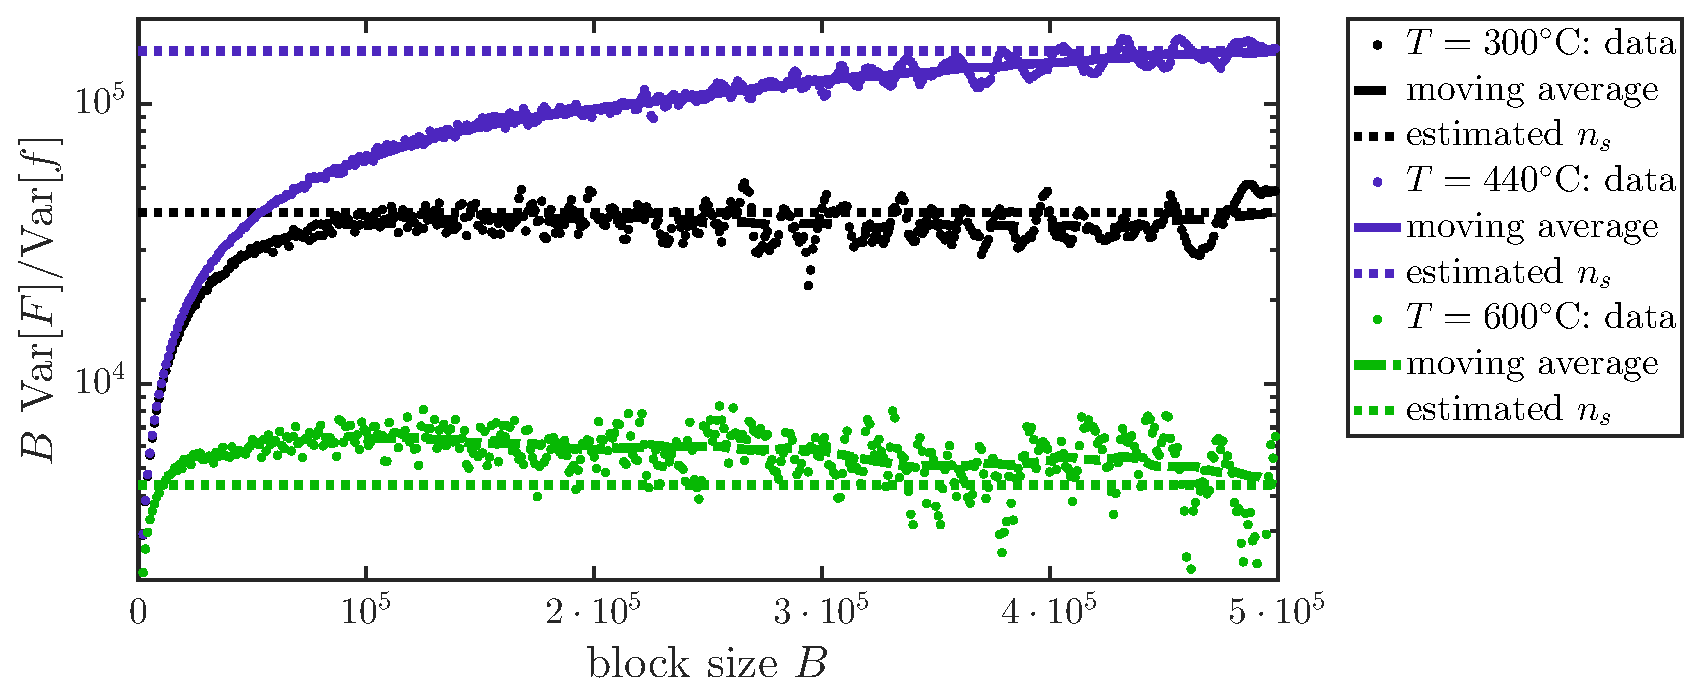
\includegraphics[width=\textwidth]{../figures/stat_inefficiency_block} 
  \caption{The statistical inefficiency determined with block averages for three different temperatures. Raw data is shown with dots, solid line show a moving average with 100 points, and the dotted lines show the estimated values of the statistical inefficiency.}
  \label{fig:ns_block}
\end{center}
\end{figure}

Note in figures~\ref{fig:ns_phi} and~\ref{fig:ns_block} that the statistical inefficiency is larger close to the phase transition at $T \approx \unit[440]{^\circ C}$ than at the lower and higher temperatures  $T = \unit[300]{^\circ C}$ and $T = \unit[600]{^\circ C}$. We speculate that this is related to the diverging property of the correlation length close to the phase transition. 

This peak in the statistical inefficiency close to the phase transition can be clearly identified also in figure~\ref{fig:ns_both}, where $n_s$ is plotted as a function of temperature using the two methods described above. We note that both methods give consistent estimates of $n_s$, but the correlation function give larger fluctuations than the block average method. Moreover, that the statistical inefficiency diverges as $T \rightarrow \unit[0]{K}$. This is because very few changes in the lattice will be accepted at low temperatures, resulting in highly correlated data. At low temperatures, the equilibrium system is almost completely ordered, and therefore the uncertainty of the quantities $U, P$ and $r$ is still small at low temperatures; note the vanishing $2-\sigma$ error bars in figures~\ref{fig:U}-\ref{fig:r}. 

\begin{figure}[!ht]
\begin{center}
  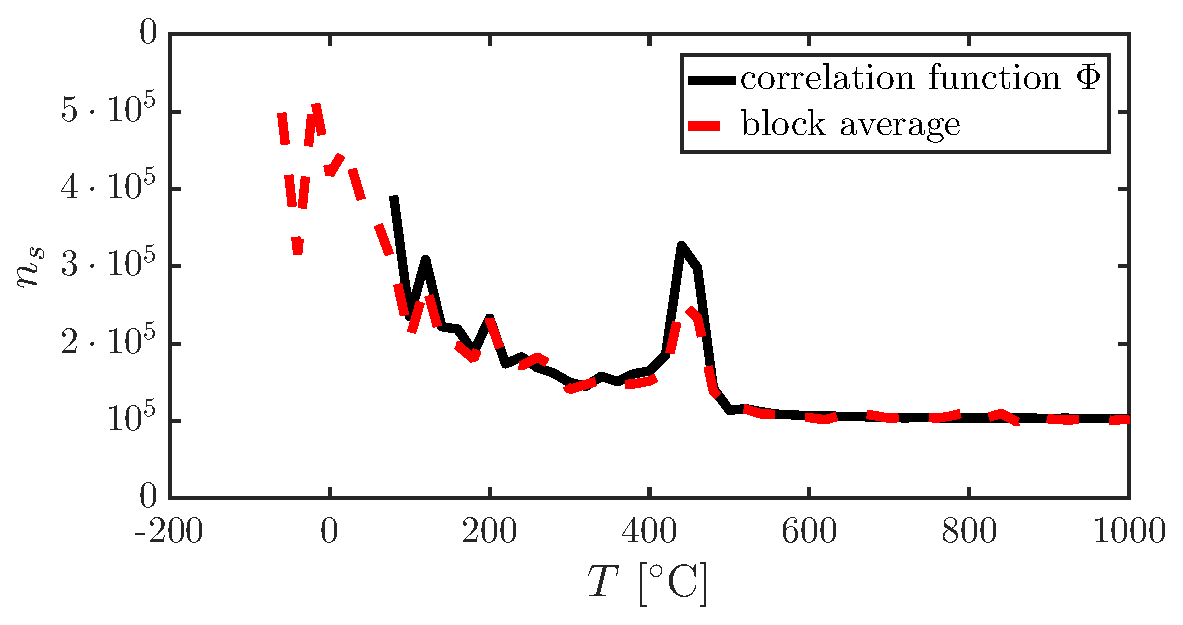
\includegraphics[width=0.7\textwidth]{../figures/stat_inefficiency_both} 
  \caption{The statistical inefficiency $n_s$ as a function of temperature using both the correlation function and block averages to determine $n_s$.}
  \label{fig:ns_both}
\end{center}
\end{figure}
\section*{Concluding discussion}
We study a binary alloy of brass. We compare semi-analytical results from mean-field theory with a Monte Carlo simulation using the Metropolis algorithm, and determine the energy, heat capacity, the order parameter as well as the short range order parameter. 

We find that the mean field theory overestimates the critical temperature. Furthermore, it fails to explain the behavior of the system above this phase transition, as the simulations show a slower convergence to the high-temperature behavior. This results in a non-zero heat capacity at supercritical temperatures, as well as a non-zero short range order parameter $r$. We also determine the critical exponents associated with the order parameter $P$ and the heat capacity from the simulations. Although these are uncertain, it is clear that they differ significantly from the mean field theory prediction. 


Finally, we consider the statistical inefficiency. The block average method is consistent with the results using the correlation function, and we observe a peak in close to the phase transition, which is possibly connected to the longer correlation length of a system close to the phase transition. 

\newpage

\appendix

\section{Source Code}

%\subsection{Calculating pi using matlab: \texttt{pi.m}}
%\lstinputlisting[language=matlab,numbers=left]{template_files/pi.m}

%\subsection{Calculating pi using python: \texttt{pi.py}}
%\lstinputlisting[language=python,numbers=left]{template_files/pi.py}

\subsection{Main program task 2: \texttt{main\_T2.c}}
\lstinputlisting[language=c,numbers=left]{../code/main_T2.c}


\subsection{Misc functions : \texttt{funcs.c}}
\lstinputlisting[language=c,numbers=left]{../code/funcs.c}

\section{Auxiliary }
\subsection{Makefile}
\lstinputlisting[language=bash,numbers=left]{../code/Makefile}

\section{MATLAB scripts}
\subsection{Task 1 and analysis scripts for Task 2}
\lstinputlisting[language=matlab,numbers=left]{../m_scripts/H2_analysis.m}

\subsection{Improve figure appearance: \texttt{ImproveFigureCompPhys.m}}
\lstinputlisting[language=matlab,numbers=left]{../m_scripts/ImproveFigureCompPhys.m}

\subsection{Change size of figures: \texttt{setFigureSize.m}}
\lstinputlisting[language=matlab,numbers=left]{../m_scripts/setFigureSize.m}
\end{document}

%%% Local Variables:
%%% mode: latex
%%% TeX-master: t
%%% End:

%  LocalWords:  MFT Helmholz's Ising
